\documentclass[13pt]{beamer}
%
% Choose how your presentation looks.
%
% For more themes, color themes and font themes, see:
% http://deic.uab.es/~iblanes/beamer_gallery/index_by_theme.html
%
\mode<presentation>
{
\usetheme{CambridgeUS}     % or try Darmstadt, Madrid, Warsaw, ...
\usecolortheme{beaver} % or try albatross, beaver, crane, ...
\usefonttheme{default}  % or try serif, structurebold, ...
\setbeamertemplate{navigation symbols}{}
\setbeamertemplate{caption}[numbered]
} 

\usepackage[english]{babel}
\usepackage[utf8x]{inputenc}
\usepackage{xcolor}
\usepackage{multicol}
\usepackage{tikz}
\usepackage{tikz-uml}
\tikzumlset{font=\footnotesize\ttfamily}
\usepackage{hyperref}

\usepackage{listings}
\definecolor{codegreen}{rgb}{0,0.6,0}
\definecolor{codegray}{rgb}{0.5,0.5,0.5}
\definecolor{codepurple}{rgb}{0.58,0,0.82}
\definecolor{backcolour}{rgb}{0.95,0.95,0.92}

\lstdefinestyle{myCustomCppStyle}{
language=C++,
numbers=left,
stepnumber=1,
numbersep=9pt,
tabsize=2,
showspaces=false,
showstringspaces=false
}

\lstset{basicstyle=\tiny,style=myCustomCppStyle}

\lstdefinestyle{mystyle}{
backgroundcolor=\color{backcolour},   
commentstyle=\color{codegreen},
keywordstyle=\color{magenta},
numberstyle=\tiny\color{codegray},
stringstyle=\color{codepurple},
basicstyle=\ttfamily\footnotesize,
breakatwhitespace=false,         
breaklines=true,                 
captionpos=b,                    
keepspaces=true,                 
numbers=left,                    
numbersep=5pt,                  
showspaces=false,                
showstringspaces=false,
showtabs=false,                  
tabsize=1
}

\lstset{style=mystyle}

\usepackage{graphicx}
\graphicspath{ {./images/} }

\usepackage{tikz}
\usetikzlibrary{decorations.text}
\usetikzlibrary{shapes.geometric, arrows, positioning, calc, matrix}

\tikzset{
basic box/.style={
shape=rectangle, rounded corners, align=center,
draw=#1, fill=#1!25},
header node/.style={
Minimum Width=header nodes,
font=\strut\Large\ttfamily,
text depth=+0pt,
fill=white, draw},
header/.style={%
inner ysep=+1.5em,
append after command={
\pgfextra{\let\TikZlastnode\tikzlastnode}
node [header node] (header-\TikZlastnode) at (\TikZlastnode.north) {#1}
node [span=(\TikZlastnode)(header-\TikZlastnode)] at (fit bounding box) (h-\TikZlastnode) {}
}
},
hv/.style={to path={-|(\tikztotarget)\tikztonodes}},
vh/.style={to path={|-(\tikztotarget)\tikztonodes}},
fat blue line/.style={ultra thick, blue}
}

\definecolor{mygray}{RGB}{208,208,208}
\definecolor{mymagenta}{RGB}{226,0,116}
\newcommand*{\mytextstyle}{\sffamily\Large\bfseries\color{black!85}}
\newcommand{\arcarrow}[3]{%
% inner radius, middle radius, outer radius, start angle,
% end angle, tip protusion angle, options, text
\pgfmathsetmacro{\rin}{1.7}
\pgfmathsetmacro{\rmid}{2.2}
\pgfmathsetmacro{\rout}{2.7}
\pgfmathsetmacro{\astart}{#1}
\pgfmathsetmacro{\aend}{#2}
\pgfmathsetmacro{\atip}{5}
\fill[mygray, very thick] (\astart+\atip:\rin)
                 arc (\astart+\atip:\aend:\rin)
-- (\aend-\atip:\rmid)
-- (\aend:\rout)   arc (\aend:\astart+\atip:\rout)
-- (\astart:\rmid) -- cycle;
\path[
decoration = {
 text along path,
 text = {|\mytextstyle|#3},
 text align = {align = center},
 raise = -1.0ex
},
decorate
](\astart+\atip:\rmid) arc (\astart+\atip:\aend+\atip:\rmid);
}
\title[Design Pattern]{Behavioral Design Pattern}
\author{Hung Tran}
\institute{Fpt software}
\date{\today}


\begin{document}

\begin{frame}
\titlepage
\end{frame}

% Uncomment these lines for an automatically generated outline.
\begin{frame}{Outline}
\tableofcontents
\end{frame}

\section{Behavioral Pattern Overview}

\begin{frame}{Behavioral Pattern Overview}
	\begin{center}
	\textcolor{blue}{\textbf{Behavioral design patterns are concerned with algorithms and the assignment of responsibilities between objects.}}
	\end{center}
	\begin{itemize}
		\item \textbf{Chain of responsibility}: lets you pass requests along a chain of handlers.
		\item \textbf{Command}: turns a request into a stand-alone object that contains all information about the request.
		\item \textbf{Iterator}: lets you traverse elements of a collection without exposing its underlying representation (list, stack, tree, etc.).
		\item \textbf{Mediator}: lets you reduce chaotic dependencies between objects.
		\item \textbf{Memento}: lets you save and restore the previous state of an object without revealing the details of its implementation.
	\end{itemize}
\end{frame}

\begin{frame}{Behavioral Pattern Overview}
	\begin{itemize}
		\item \textbf{Observer}: lets you define a subscription mechanism to notify multiple objects about any events that happen to the object they’re observing.
		\item \textbf{State}: lets an object alter its behavior when its internal state changes. It appears as if the object changed its class.
		\item \textbf{Strategy}: lets you define a family of algorithms, put each of them into a separate class, and make their objects interchangeable.
		\item \textbf{Template Method}: defines the skeleton of an algorithm in the superclass but lets subclasses override specific steps of the algorithm without changing its structure.
		\item \textbf{Visitor}: lets you separate algorithms from the objects on which they operate.
	\end{itemize}
\end{frame}

\section{Chain of Responsibility pattern}

\begin{frame}{Problem Statement: online ordering system}
	\begin{columns}[T]
		\begin{column}{.5\textwidth}
			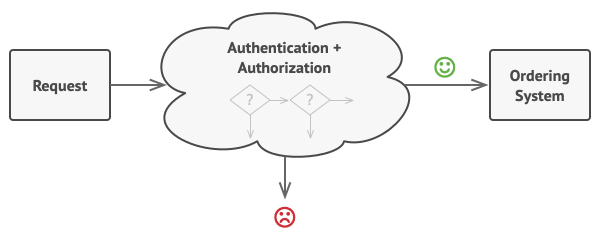
\includegraphics[scale=0.3]{./images/problem.png}
			\begin{itemize}
				\item Restrict access to the system so only authenticated users can create orders.
				\item Users who have administrative permissions must have full access to all orders.
				\item These checks must be performed sequentially.
			\end{itemize}
		\end{column}
	
		\begin{column}{.5\textwidth}
			\begin{itemize}
				\item Validation step to sanitize the data in a request.
				\item Check that filters repeated failed requests coming from the same IP address.
				\item Speed up the system by returning cached results on repeated requests containing the same data. Hence, you added another check which lets the request pass through to the system only if there’s no suitable cached response.
			\end{itemize}
		\end{column}
	\end{columns}
\end{frame}

\begin{frame}{Solution: Chain of Responsibility Pattern}
	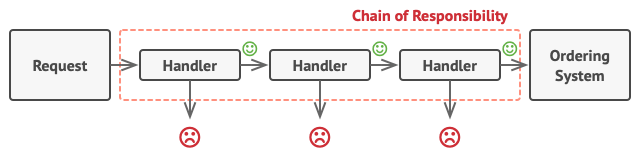
\includegraphics[scale=0.55]{./images/solution.png}
	\begin{itemize}
		\item Each check should be extracted to its own class with a single method that performs the check.
		\item Each linked handler has a field for storing a reference to the next handler.
		\item A handler can decide not to pass the request further down the chain and effectively stop any further processing
	\end{itemize}
\end{frame}

\begin{frame}{The Intent of Chain of Responsibility Design Pattern}
	\begin{center}
	\textcolor{red}{\textbf{Chain of Responsibility is a behavioral design pattern that lets you pass requests along a chain of handlers. Upon receiving a request, each handler decides either to process the request or to pass it to the next handler in the chain.}}\\
	\end{center}
\end{frame}

\begin{frame}{Structure of Chain of Responsibility Pattern}
	\begin{center}
	\begin{tikzpicture}
 	\umlemptyclass[x=0,y=0]{Client}
 	\umlclass[x=5,y=0]{Handler}{-nextHandler}{+handlerRequest() \\ +setNextHandler()}
 	\umlclass[x=3,y=-4]{ConcreteHandle1}{}{+handlerRequest()}
 	\umlclass[x=7,y=-4]{ConcreteHandle2}{}{+handlerRequest()}
 	\umluniassoc[pos=0.95, align=right, name=uniassoc]{Client}{Handler}
 	\umlinherit[geometry=|-|, pos=0.95, align=right, name=uniassoc]{ConcreteHandle1}{Handler}
 	\umlinherit[geometry=|-|, pos=0.95, align=right, name=uniassoc]{ConcreteHandle2}{Handler}
	\end{tikzpicture}	
	\end{center}
\end{frame}

\begin{frame}{Sequence Diagram}
\begin{center}
	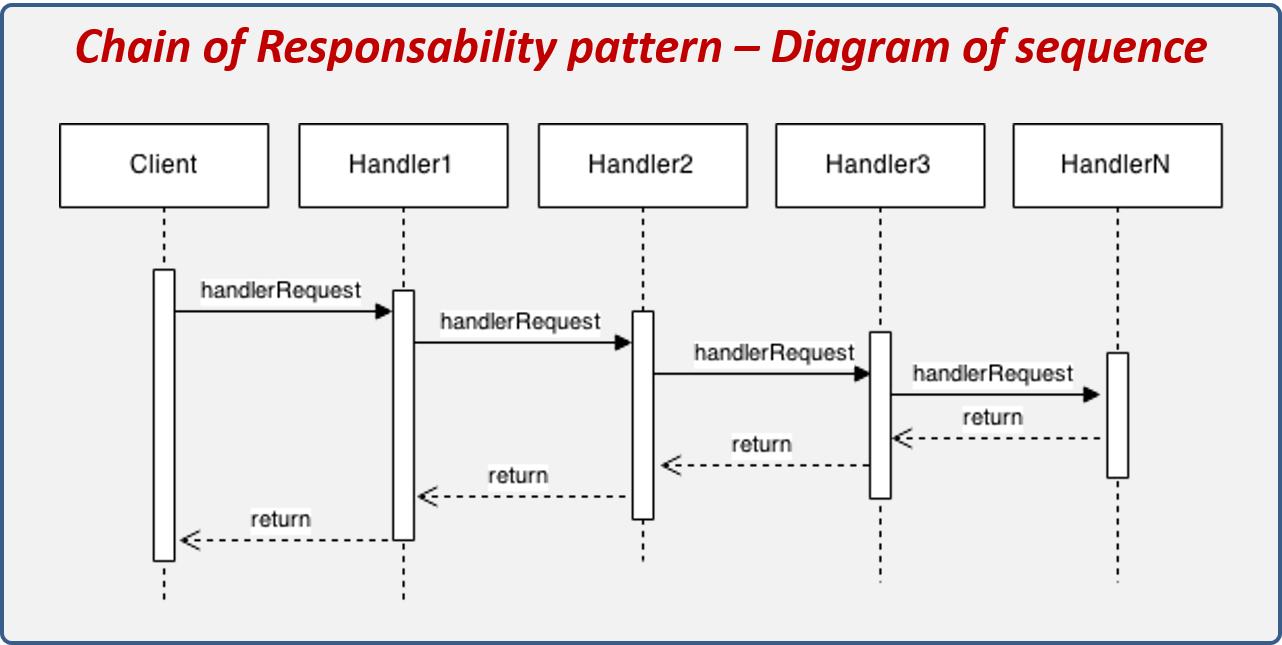
\includegraphics[scale=0.25]{./images/sequence.png}
\end{center}
\end{frame}

\begin{frame}{Basic implementation: handler class}
\begin{columns}[T]
\begin{column}{.45\textwidth}
\lstset{basicstyle=\tiny,style=myCustomCppStyle}
handler.h
\lstinputlisting{./examples/handler.h}
\end{column}

\begin{column}{.45\textwidth}
\lstset{basicstyle=\tiny,style=myCustomCppStyle}
handler.cpp
\lstinputlisting{./examples/handler.cpp}
\end{column}
\end{columns}
\end{frame}

\begin{frame}{Basic implementation: concreteHandler1 class}
\begin{columns}[T]
\begin{column}{.45\textwidth}
\lstset{basicstyle=\tiny,style=myCustomCppStyle}
concreteHandler1.h
\lstinputlisting{./examples/concreteHandler1.h}
\end{column}

\begin{column}{.45\textwidth}
\lstset{basicstyle=\tiny,style=myCustomCppStyle}
concreteHandler1.cpp
\lstinputlisting{./examples/concreteHandler1.cpp}
\end{column}
\end{columns}
\end{frame}

\begin{frame}{Basic implementation: concreteHandler2 class}
\begin{columns}[T]
\begin{column}{.45\textwidth}
\lstset{basicstyle=\tiny,style=myCustomCppStyle}
concreteHandler2.h
\lstinputlisting{./examples/concreteHandler2.h}
\end{column}

\begin{column}{.45\textwidth}
\lstset{basicstyle=\tiny,style=myCustomCppStyle}
concreteHandler2.cpp
\lstinputlisting{./examples/concreteHandler2.cpp}
\end{column}
\end{columns}
\end{frame}

\begin{frame}{Basic implementation: main}
\begin{columns}[T]
\begin{column}{.45\textwidth}
\lstset{basicstyle=\tiny,style=myCustomCppStyle}
main.cpp
\lstinputlisting{./examples/main.cpp}
\end{column}

\begin{column}{.45\textwidth}
\end{column}
\end{columns}
\end{frame}

\begin{frame}{Applicability}
	\begin{itemize}
		\item  When we can conceptualize our program as a chain made up of links, where each link can either handle a request or pass it up the chain.
		\item When we want to decouple a request’s sender and receiver.
		\item Multiple handlers determined at runtime.
		\item More than one object may handle a request, and the handler is not known in advance.
		\item The handler should be ascertained automatically.
		\item We may want to issue a request to one of several objects without specifying the receiver explicitly.
		\item The set of handlers that can handle a request should be specified dynamically.
		\item A scenario within you need to pass a request to one handler among a list of handlers at run-time based on certain conditions.
	\end{itemize}
\end{frame}

\begin{frame}{How to Implement}
	\begin{itemize}
		\item Declare the handler interface and describe the signature of a method for handling requests.
		\item To eliminate duplicate boilerplate code in concrete handlers, it might be worth creating an abstract base handler class, derived from the handler interface.
		\item One by one create concrete handler subclasses and implement their handling methods. Each handler should make two decisions when receiving a request:.
		\item The client may either assemble chains on its own or receive pre-built chains from other objects. In the latter case, you must implement some factory classes to build chains according to the configuration or environment settings.
		\item The client may trigger any handler in the chain, not just the first one. The request will be passed along the chain until some handler refuses to pass it further or until it reaches the end of the chain.
	\end{itemize}
\end{frame}

\begin{frame}{Pros and Cons}
	\begin{columns}[T]
		\begin{column}{.5\textwidth}
			\begin{itemize}
				\item You can control the order of request handling.
				\item Single Responsibility Principle. You can decouple classes that invoke operations from classes that perform operations.
				\item Open/Closed Principle. You can introduce new handlers into the app without breaking the existing client code.
			\end{itemize}
		\end{column}
	
		\begin{column}{.5\textwidth}
			\begin{itemize}
				\item Some requests may end up unhandled.
			\end{itemize}
		\end{column}
	\end{columns}
\end{frame}

\begin{frame}{Relations with Other Patterns}
	\begin{itemize}
		\setlength\itemsep{1em}
		\item Chain of Responsibility, Command, Mediator and Observer address various ways of connecting senders and receivers of requests:
		\item Chain of Responsibility is often used in conjunction with Composite. In this case, when a leaf component gets a request, it may pass it through the chain of all of the parent components down to the root of the object tree.
		\item Handlers in Chain of Responsibility can be implemented as Commands. In this case, you can execute a lot of different operations over the same context object, represented by a request.
		\item Chain of Responsibility and Decorator have very similar class structures. Both patterns rely on recursive composition to pass the execution through a series of objects. However, there are several crucial differences.
	\end{itemize}
\end{frame}

\begin{frame}
\begin{center}
{\fontsize{40}{50}\selectfont Thank You!}
\end{center}
\end{frame}

\end{document}
